\section{Method}
\label{sec:method}

\subsection{Background}

\paragraph{Speculative decoding.}
At each iteration, $M_d$ samples a length-$k$ continuation
$\hat{x}_{t+1:t+k} \sim \prod_{i=1}^{k} q(x_{t+i} \mid x_{\le t+i-1})$
from prefix $x_{\le t}$. $M_t$ then computes
$p(x_{t+i} \mid x_{\le t+i-1})$ for $i = 1,\dots,k+1$ in a single
forward pass over $k+1$ positions. Each drafted token is accepted with
probability $\min(1, p/q)$, the first rejection is resampled from the
residual distribution, and decoding resumes. Samples are exactly
distributed according to $p$~\cite{leviathan2023, chen2023}.

\paragraph{Speculative$^2$ decoding.}
S$^2$D~\cite{saguaro2024} observes that in vanilla SD, $M_d$ sits idle
while $M_t$ verifies. Instead, while $M_t$ verifies block $b$, $M_d$
\emph{simultaneously} predicts what the verifier is likely to accept
and drafts continuations for each of the $f$ most probable verification
outcomes. If the verifier's outcome lies in this tree (common at high
acceptance rate), the next draft block is already prepared; otherwise
the engine falls back to a recovery draft.

\paragraph{Discrete diffusion drafters.}
MDLM~\cite{sahoo2024} parameterizes $p_\theta(x_0 \mid x_t)$ where
$x_t$ is partially masked. At inference time we start from a fully
masked block and iteratively unmask high-confidence positions over $R$
refinement steps, with $R \ll k$. BD3LM~\cite{arriola2025} additionally
imposes a \emph{block-causal} attention structure (the staircase
pattern): positions in block $b$ may attend to earlier blocks plus
positions inside block $b$, but not to future blocks.

\subsection{Diffusion drafting inside S$^2$D}

We add a \texttt{block} draft backend
(\texttt{BlockDiffusionDraftBackend} in
\texttt{ssd/engine/draft\_backends.py}) that replaces the AR drafter in the
S$^2$D loop. For a batch of sequences with prefixes
$\{x^{(b)}_{\le t_b}\}_{b=1}^{B}$ and a requested lookahead $k$, the
backend executes the following:

\begin{enumerate}
  \item \textbf{Prepare input.} For each sequence, allocate a buffer of
        length $t_b + k$, fill the prefix region with $x^{(b)}_{\le t_b}$,
        and the next $k$ positions with the mask token
        $\mathsf{m}$. Pad the batch to a common length.
  \item \textbf{Refine for $R$ steps.} At each step
        $r = 0, \dots, R-1$, run a forward pass of the diffusion model,
        extract the $k$ block logits, project them onto the target
        vocabulary, and run the configured sampler (Sec.~\ref{sec:samplers})
        to update the block.
  \item \textbf{Emit draft.} After step $R-1$, the block contains the
        proposed draft tokens. We return both the tokens and the final
        block logits, which S$^2$D uses for the speculation tree.
\end{enumerate}

The verifier then proceeds exactly as in standard S$^2$D, treating the
diffusion-generated block like any other length-$k$ draft. Acceptance is
performed token-by-token along the block, so distributional correctness
relative to $M_t$ is inherited from the underlying SD rejection rule.

\subsection{Samplers and attention modes}
\label{sec:samplers}

We implement three samplers that govern \emph{which} masked positions get
committed at each refinement step. Let
$\pi_i = \mathrm{softmax}(\mathrm{logits}_i)$ and
$\hat{x}_i = \arg\max_v \pi_{i,v}$ be the per-position argmax, with
confidence $c_i = \max_v \pi_{i,v}$.

\begin{itemize}
  \item \textbf{Mask-predict.} At step $r$, lock the
        $\lceil k \cdot (r+1)/R \rceil$ highest-confidence positions to
        $\hat{x}_i$; re-mask the rest. Variant of~\cite{ghazvininejad2019}.
  \item \textbf{Remask.} Commit all argmax tokens, then re-mask the
        $k - \lceil k(r+1)/R\rceil$ \emph{least} confident positions. This
        is the original MDLM-style sampler.
  \item \textbf{First-hitting.} Compatible only with staircase attention.
        At step $r$, commit a fixed schedule of $s_r$ tokens chosen by
        confidence and never re-mask them. This matches the BD3LM
        decoding rule.
\end{itemize}

Attention is one of \texttt{full} (bidirectional within the whole sequence,
as in MDLM) or \texttt{staircase} (block-causal, as in BD3LM). When the
staircase pattern is used and the prefix is stable across draft calls, we
optionally maintain a per-sequence prefix KV cache (\texttt{block\_prefix\_cache})
keyed by the longest common prefix of consecutive calls, so that only the
masked block is forwarded through the model each refinement step.

\subsection{AR warm-start and switching}

Diffusion drafters are most useful once the prefix is long enough to
give the block model meaningful conditioning context; early in a
generation the prefix is short and the diffusion drafter under-performs
a tiny AR drafter. We therefore wrap two backends in a
\texttt{SwitchingDraftBackend}: an AR drafter handles the first $N$
completion tokens, after which the block-diffusion drafter takes over.
On single-GPU servers the inactive backend is paged out by default;
\texttt{--block-warm-start-keep-loaded} keeps both resident on
multi-GPU machines where memory is not the binding constraint.

The pipeline is implemented in a custom inference engine that also
supports tensor parallelism, PagedAttention, CUDA graphs,
\texttt{torch.compile}, and target-side prefix caching. Sync SD and
async S$^2$D share the same draft backend interface, so the diffusion
drafter slots in unchanged; the block backend is currently restricted
to sync SD, with async support a natural next step. Code lives in
\texttt{ssd/engine/draft\_backends.py} and is exposed by
\texttt{bench.py} via \texttt{--draft-backend block}.

\begin{figure*}[t]
  \centering
  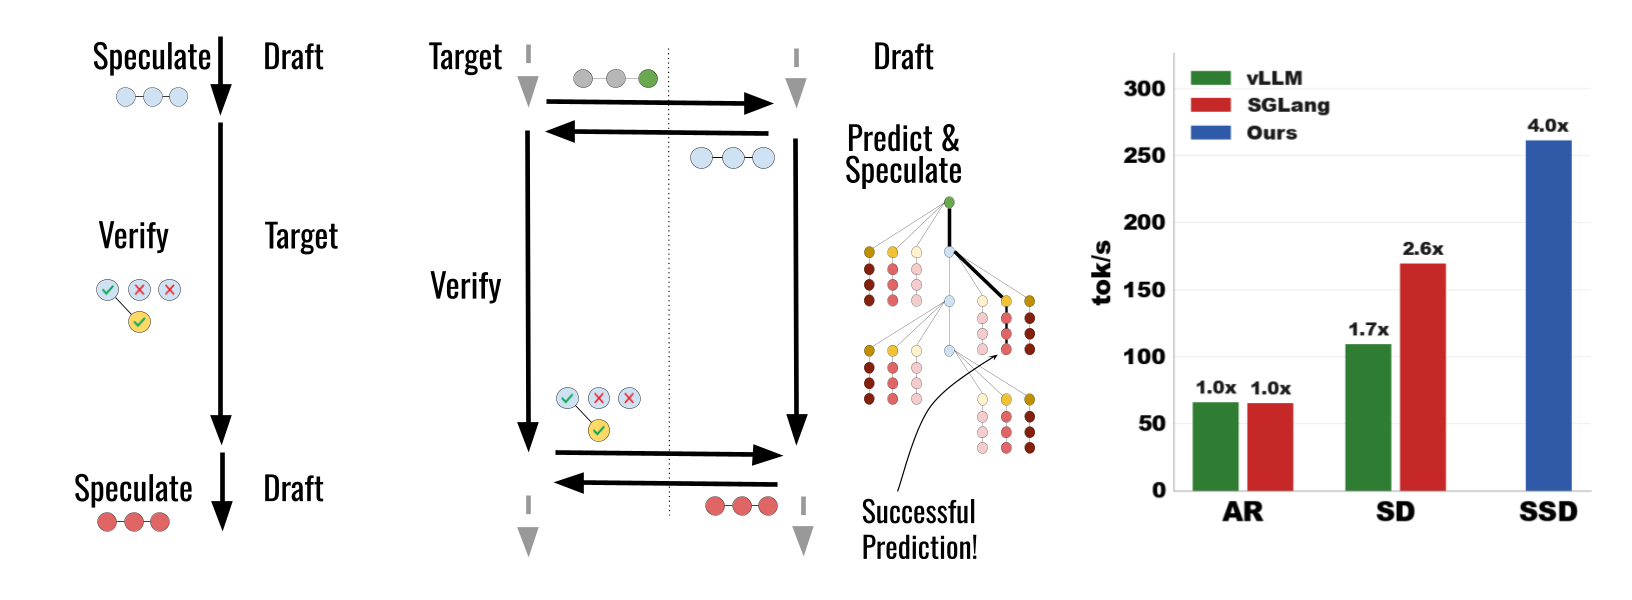
\includegraphics[width=0.95\linewidth]{overview.png}
  \caption{
    \textbf{Left:} standard speculative decoding alternates draft and
    verify on the same hardware, so the draft model is idle during
    verification. \textbf{Middle:} S$^2$D runs draft and verify in
    parallel by speculating against multiple predicted verification
    outcomes; on a hit (green leaf) the next block is already in hand.
    \textbf{Right:} this work replaces the AR drafter inside the S$^2$D
    loop with a discrete diffusion drafter that fills an entire block in
    $R$ parallel refinement steps. The bar chart shows headline tokens/s
    on \texttt{Llama-3.3 70B} with AR, SD, and S$^2$D drafts; the empty
    slot for ``diffusion-S$^2$D'' is the target of this work.
  }
  \label{fig:overview}
\end{figure*}
